\documentclass[pdflatex,iicol,sn-mathphys-ay]{sn-jnl}

\usepackage[T1]{fontenc}
\usepackage[utf8]{inputenc}
\usepackage[english]{babel}
\usepackage{amsmath,amssymb,amsthm,bm}
\usepackage{booktabs}
\usepackage{graphicx}
\usepackage{tikz}
\usepackage{placeins}
\usepackage{microtype}
\usepackage{siunitx}
\usepackage[nameinlink,noabbrev]{cleveref}
\newtheorem{proposition}{Proposition}
\newtheorem{theorem}{Theorem}
\raggedbottom

\graphicspath{{figures/}}
% Generated by scripts/generate_results.m.
\newcommand{\NominalPeriodMicroseconds}{286}
\newcommand{\NominalIntervalCount}{9}
\newcommand{\NominalClosureError}{1.421e-14}
\newcommand{\NominalMinimumDwell}{22.000}
\newcommand{\BenchmarkDwellBound}{22}
\newcommand{\AppliedScheduleDwellBound}{3}
\newcommand{\MaximumBoundaryCorrection}{2.111}
\newcommand{\CycleAverageVCOne}{10.41056}
\newcommand{\CycleAverageVCTwo}{19.42228}
\newcommand{\CycleAverageIL}{0.95613}
\newcommand{\TimingScaleMicroseconds}{10}
\newcommand{\PhiJacobianRelativeError}{8.518e-12}
\newcommand{\GammaJacobianRelativeError}{8.344e-11}
\newcommand{\LinearizationResidualSlope}{2.000}
\newcommand{\OpenLoopSpectralRadius}{0.999850}
\newcommand{\ConservativeSpectralRadius}{0.941468}
\newcommand{\AggressiveSpectralRadius}{0.568151}
\newcommand{\InvariantRegionFacets}{7}
\newcommand{\InvariantRegionVertices}{10}
\newcommand{\InvariantRegionVolume}{4.5410}
\newcommand{\InvariantRegionVCOneMin}{-2.358}
\newcommand{\InvariantRegionVCOneMax}{2.098}
\newcommand{\InvariantRegionVCTwoMin}{-3.234}
\newcommand{\InvariantRegionVCTwoMax}{1.911}
\newcommand{\InvariantRegionILMin}{-0.496}
\newcommand{\InvariantRegionILMax}{0.222}
\newcommand{\InvariantRegionIterations}{1}
\newcommand{\InvariantRegionImageDwellMargin}{4.347}
\newcommand{\FirstInvariantRegionCycle}{3}
\newcommand{\LowerComparisonConditioningFactor}{0.25}
\newcommand{\MiddleComparisonConditioningFactor}{0.5}
\newcommand{\LowerComparisonRegionVolume}{290.6254}
\newcommand{\MiddleComparisonRegionVolume}{36.3282}
\newcommand{\LowerComparisonRegionVolumeRatio}{64}
\newcommand{\MiddleComparisonRegionVolumeRatio}{8}
\newcommand{\AggressiveInputWeight}{0.001}
\newcommand{\ConservativeInputWeight}{0.1}
\newcommand{\InitialNormalizedError}{0.983946}
\newcommand{\ConditionedFinalError}{1.746e-15}
\newcommand{\ConservativeFinalError}{3.113e-06}
\newcommand{\OpenLoopFinalError}{0.298010}
\newcommand{\ConditionedSettlingCycle}{6}
\newcommand{\ConservativeSettlingCycle}{20}
\newcommand{\ConditionedCycleCount}{3}
\newcommand{\MinimumConditioningBeta}{0.293978}
\newcommand{\MaximumRawOffset}{65.217}
\newcommand{\MaximumAppliedOffset}{19.172}
\newcommand{\MinimumRawDwell}{-43.045}
\newcommand{\MinimumAppliedDwell}{3.000}
\newcommand{\MinimumConservativeDwell}{15.502}
\newcommand{\SimulationCycles}{100}
\newcommand{\LongSimulationCycles}{100000}
\newcommand{\OpenLoopConvergenceCycle}{22009}

% Generated by paper.export_lyapunov from the Julia certificate.
\newcommand{\LyapunovEta}{2.911904315e-04}
\newcommand{\LyapunovMinEigenvalue}{4.987946970e-03}
\newcommand{\LyapunovEndpointZeroDecrease}{2.911904317e-04}
\newcommand{\LyapunovEndpointOneDecrease}{2.911956096e-04}
\newcommand{\LyapunovDecrease}{2.911904317e-04}
\newcommand{\LyapunovRateBound}{0.999938954110}
\newcommand{\LyapunovMatrix}{\begin{bmatrix}
0.608770 & -0.013731 & 0.027354\\
-0.013731 & 2.384502 & 0.033889\\
0.027354 & 0.033889 & 0.006728
\end{bmatrix}}

% Generated by studies/beta-timing/export_latex.py; do not edit.
% Source: studies/beta-timing/results/summary.csv and environment metadata.
% Individual-call p95 and p95 of batch-average costs are distinct statistics.
% summary.csv SHA256: d4e83d83b9da82289b3e5db8acfca18d601852b0dc1958971eeadbc238f2f150
\newcommand{\BetaTimingCpu}{AMD Ryzen 7 7800X3D 8-Core Processor}
\newcommand{\BetaTimingMatlabRelease}{2025b}
\newcommand{\BetaTimingGccVersion}{13.2.0}
\newcommand{\BetaTimingWarmupCalls}{5000}
\newcommand{\BetaTimingIndividualSamples}{10000}
\newcommand{\BetaTimingBatchSamples}{500}
\newcommand{\BetaTimingBatchSize}{200}
\newcommand{\BetaTimingInputCount}{100}
\newcommand{\BetaTimingMatlabBetaPninetyfiveUs}{3.6}
\newcommand{\BetaTimingMatlabFullPninetyfiveUs}{5.3}
\newcommand{\BetaTimingMatlabActiveBetaPninetyfiveUs}{3.2}
\newcommand{\BetaTimingMatlabActiveFullPninetyfiveUs}{3.9}
\newcommand{\BetaTimingCppTimerFloorUs}{0.1}
\newcommand{\BetaTimingCppBetaBatchPninetyfiveNs}{7.5}
\newcommand{\BetaTimingCppFullBatchPninetyfiveNs}{25.5}

% Generated from checked 1x MPC evidence and matched host timing.
\newcommand{\MpcHorizon}{5}
\newcommand{\ProposedEvaluationCost}{1.54565}
\newcommand{\MpcEvaluationCost}{1.30990}
\newcommand{\MpcCostReduction}{15.3}
\newcommand{\MpcSettlingCycle}{5}
\newcommand{\MpcSettlingMilliseconds}{1.430}
\newcommand{\ProposedMatchedMedianUs}{6.70}
\newcommand{\MpcMatchedMedianUs}{230.70}
\newcommand{\ProposedMatchedPninetyfiveUs}{10.90}
\newcommand{\MpcMatchedPninetyfiveUs}{603.45}
\newcommand{\MatchedTimingSamples}{5760}
\newcommand{\MatchedTimingWarmup}{1008}
\newcommand{\MatchedTimingStates}{24}
\newcommand{\MatchedTimingMatlabRelease}{2025b}


\newcommand{\R}{\mathbb{R}}
\newcommand{\vect}[1]{\bm{#1}}
\newcommand{\dtau}{\delta\vect{\tau}}
\newcommand{\ddwell}{\delta\vect{d}}
\newcommand{\X}{\mathcal{X}}

\begin{document}

\title[Dwell-conditioned switching-time feedback]{Dwell-Conditioned Cycle-to-Cycle Switching-Time Feedback for Mode-Dependent Switched-Affine Systems}

\author*[1]{\fnm{Daniel} \sur{Vieira}}\email{danielvie@gmail.com}
\author[1]{\fnm{Roberto Kawakami Harrop} \sur{Galv\~ao}}

\affil*[1]{\orgdiv{Systems and Control}, \orgname{Instituto Tecnol\'ogico de Aeron\'autica}, \orgaddress{\city{S\~ao Jos\'e dos Campos}, \state{S\~ao Paulo}, \country{Brazil}}}

\abstract{
This paper adresses the problem of controlling a switching-time affine system under dwell-time constraints. The goal is to steer the system to a target periodic trajectory rather than a constant average operating point. We propose a proportional controller and a signal conditioner to comply with the minimum dwell-time constraints. The method combines a solver-free enforcement of the minimum dwell-time constraints with a common quadratic Lyapunov function approach. The controller acts by generating the delta time to be applyed on the switching instants, then conditioning the signal by reducing the requested adjustiments when the schedule is not feasible. The example used here is a three-cell DC-DC converter, we verify the stability of the linearized model using this approach. The simulations show faster convergence of this method compared to a conservative feedback and open-loop opearation while respecting the dwell-time contraints. The analysis guarantees exponential stability of the lineared model even when the conditioning factor changes from cyclo to other.
}

\keywords{switched-affine systems, periodic trajectories, switching-time control, dwell-time conditioning, common quadratic Lyapunov function, semidefinite programming}

\maketitle

\section{Introduction}

Power converters control voltage and current by moving through a sequence of switch configurations. The switching pattern must respect electrical limits, switching frequency, a minimum dwell duration for transition, and a short computation time \cite{karamanakos2020mpcPowerElectronics}. Keeping the individual configurations explicit gives a hybrid-affine or switched-affine model \cite{albea2021hybridAffinePwm}. When repeating the pattern, then it produces a periodic trajectory rather than a constant state, and controlling such trajectories is an established problem for switched-affine systems \cite{egidio2020,xu2024fcsLimitCycle}.

Predictive control tackles the problem by solving a constrained optimization problem online. Recent work reduces the online burden through Laguerre parameterization, dedicated fixed-frequency solvers, and candidate pruning \cite{saeed2022laguerre,yang2022fixed,augustine2023mpc}. Controllers also differ in what they may change. State-dependent switching laws choose the active subsystem \cite{egidio2022rank}, where switching-time control keeps an ordered sequence and moves its transition instants. We take this same approach by changing the transition instants while keeping all other parameters fixed. At each cycle start, the error is computed and the offsets applied during that cycle, with no online solver.

Fixed-period switching-time control shifts only the interior switching instants without changing the mode sequence or cycle period. It targets a reference periodic trajectory rather than an equilibrium point. Patino et al. studied how individual switching instants affect mode-dependent cyclic systems and used predictive control to track an optimal periodic trajectory \cite{patino2010}. Marcolino et al. regulated the cycle-start state toward a target point on the periodic trajectory, referred to in this paper as the cycle anchor. For a fixed-period linear model with switched actuator levels, they used a one-cycle model to compute switching-instant corrections through discrete LQR and dwell-constrained predictive control \cite{marcolino2021}. Shifting a switching instant makes the preceding dwell duration larger and the following one shorter, coupling their minimum-dwell constraints. Marcolino et al. enforce these constraints through online optimization in their predictive controller. Their LQR method instead clips each adjustment separately to meet the dwell limits. This can change the direction of the requested adjustments and may shift the final switching instant \cite{marcolino2021}. Preserving the direction of the control action through control allocation still requires online optimization and does not address fixed-period dwell constraints \cite{nakamuraZimmerer2026directionPreserving}. The remaining problem is to compute the largest feasible scale without an online solver. The scale must preserve the action direction and mode order without changing the cycle period.

To make fixed-period switching-time feedback dwell-feasible, we scale every requested offset by the same factor, taking the smallest of $1$ and the bounds imposed by the $N$ dwell constraints. We find this largest feasible factor in $O(N)$ time without an online solver, while scaling the full raw offset vector preserves its direction, the mode order, and the cycle period. We assess convergence separately with an offline common quadratic Lyapunov certificate, which establishes uniform exponential stability of the conditioned linearized model even when the factor changes between cycles. The conditioner makes each finite timing request dwell-feasible, but the certificate does not guarantee convergence of the exact nonlinear plant from arbitrary errors. \Cref{sec:model} derives the cycle model, \cref{sec:conditioning} develops the conditioner, \cref{sec:stability} presents the stability analysis, and \cref{sec:case-study} presents the converter study.

\section{Problem formulation and one-cycle model}
\label{sec:model}

To compute the timing action that the conditioner will scale, we first need a model of how switching-time adjustments affect tracking. With the mode sequence and cycle period fixed, we derive a linearized relation between the tracking error at the start of a cycle, the timing offsets applied during that cycle, and the error at the start of the next cycle. We then use this model to define the raw proportional feedback law.

\subsection{Plant, reference trajectory, and timing coordinates}

Consider the switched-affine plant
\begin{equation}
    \dot{\vect{x}}(t)=A_{\sigma(t)}\vect{x}(t)+\vect{b}_{\sigma(t)},
    \qquad \vect{x}(t)\in\R^n.
    \label{eq:plant}
\end{equation}
Every cycle executes the sequence $(q_1,\ldots,q_N)$. Its nominal cycle boundaries and dwell durations are
\begin{equation}
\begin{aligned}
    0&=\bar t_0<\bar t_1<\cdots<\bar t_N=T,\\
    \bar d_i&=\bar t_i-\bar t_{i-1}.
\end{aligned}
\end{equation}
The given reference schedule generates $\bar{\vect{x}}(t)$ with anchor $\bar{\vect{x}}(0)=\bar{\vect{x}}(T)$. Define $\vect{x}_k=\vect{x}(kT)$ and $\vect{e}_k=\vect{x}_k-\bar{\vect{x}}(0)$. The target is periodic motion, not a constant average operating point.

The controller moves only the $N-1$ interior switching instants, keeping the cycle endpoints fixed, as illustrated in \cref{fig:timing-mechanism}(a):
\begin{equation}
\begin{aligned}
    t_{k,i}&=\bar t_i+\delta\tau_{k,i},\quad i=1,\ldots,N-1,\\
    \delta\tau_{k,0}&=\delta\tau_{k,N}=0.
\end{aligned}
\end{equation}
During cycle $k$, mode $q_i$ is active from $kT+t_{k,i-1}$ to $kT+t_{k,i}$, so its dwell duration is $d_{k,i}=t_{k,i}-t_{k,i-1}$. Moving a boundary transfers time between its neighboring intervals. In \cref{fig:timing-mechanism}(b), delaying instant 8 by \SI{12}{\micro\second} lengthens dwell 8 by \SI{12}{\micro\second} and shortens dwell 9 by the same amount; the other dwells remain unchanged.

These transfers preserve the total period $T$, but a sufficiently large shift can reverse the boundary order, as \cref{fig:timing-mechanism}(c) illustrates. We therefore require every applied dwell to satisfy $d_{k,i}\ge d_{\min}$, where $d_{\min}>0$ is the minimum allowed dwell duration.

\begin{figure*}[t]
    \centering
    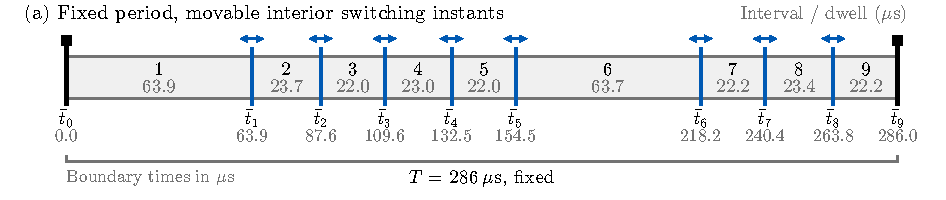
\includegraphics[width=\textwidth]{timing_coordinates.pdf}\par\smallskip
    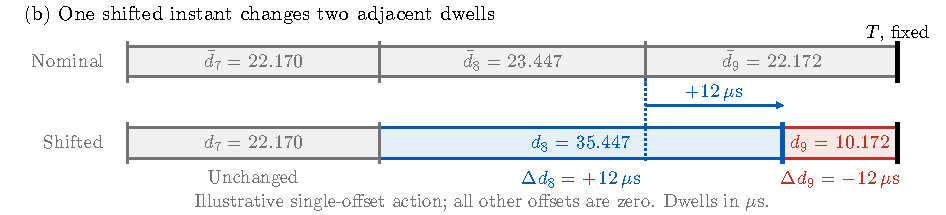
\includegraphics[width=\textwidth]{dwell_coupling.pdf}\par\smallskip
    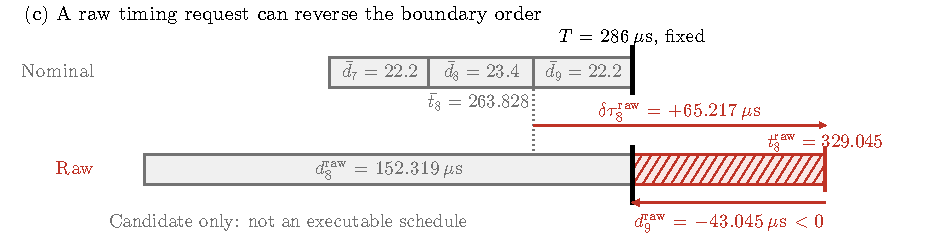
\includegraphics[width=\textwidth]{inadmissible_request.pdf}
    \caption{Switching-instant adjustments in the converter schedule of \cref{sec:case-study}. (a) Eight interior switching instants can move while the cycle endpoints remain fixed. (b) Delaying instant 8 transfers \SI{12}{\micro\second} from dwell 9 to dwell 8. (c) An inadmissible first-cycle raw request moves instant 8 beyond the cycle end. Hatching denotes the resulting negative candidate dwell.}
    \label{fig:timing-mechanism}
\end{figure*}

\subsection{Exact augmented propagation and terminal error}

The augmented state and system matrix are
\begin{equation}
    \X(t)=\begin{bmatrix}\vect{x}(t)\\1\end{bmatrix},\qquad
    \widetilde A_q=
    \begin{bmatrix}A_q&\vect{b}_q\\\vect{0}^{\mathsf T}&0\end{bmatrix}.
    \label{eq:augmented-generator}
\end{equation}
Then $\dot\X(t)=\widetilde A_{\sigma(t)}\X(t)$. Within one cycle, $t_i$ denotes $t_{k,i}$, and state arguments are relative to the cycle start. The fixed endpoints are $t_0=\bar t_0=0$ and $t_N=\bar t_N=T$, with mode $q_i$ on $[t_{i-1},t_i)$.

The interval durations satisfy
\begin{equation}
\begin{aligned}
    \Delta t_i&=t_i-t_{i-1},\\
    \Delta\bar t_i&=\bar t_i-\bar t_{i-1},\\
    \Delta t_i&=\Delta\bar t_i+\delta t_i,\qquad F_i=\widetilde A_{q_i}.
\end{aligned}
\label{eq:duration-coordinates}
\end{equation}
Thus $\Delta t_i=d_{k,i}$, $\Delta\bar t_i=\bar d_i$, and $\delta t_i=\delta d_{k,i}$ is a duration change, not an instant offset. Interval propagation is
\begin{equation}
    \X(t_i)=e^{F_i\Delta t_i}\X(t_{i-1}).
\end{equation}
Therefore, the exact cycle propagation is
\begin{equation}
    \X(t_N)=e^{F_N\Delta t_N}e^{F_{N-1}\Delta t_{N-1}}
    \cdots e^{F_1\Delta t_1}\X(t_0).
    \label{eq:exact-augmented-cycle}
\end{equation}
At the nominal duration, the interval transition matrix is
\begin{equation}
    \phi_i=e^{F_i\Delta\bar t_i}.
    \label{eq:nominal-interval-transition}
\end{equation}
The nominal augmented trajectory is $\bar\X(t)=[\bar{\vect{x}}(t)^{\mathsf T}\ 1]^{\mathsf T}$, so its terminal state satisfies
\begin{equation}
    \bar\X(t_N)=\phi_N\phi_{N-1}\cdots\phi_1\bar\X(t_0).
    \label{eq:nominal-augmented-cycle}
\end{equation}
The augmented error and initial state satisfy
\begin{equation}
\begin{aligned}
    \vect{e}(t)&=\X(t)-\bar\X(t),\\
    \X(t_0)&=\bar\X(t_0)+\vect{e}(t_0).
\end{aligned}
\end{equation}
The augmented error $\vect{e}(t)\in\R^{n+1}$ has last component zero; its first $n$ components at the cycle start form $\vect{e}_k$. At $t_N=T$, subtracting the nominal propagation gives
\begin{equation}
\begin{aligned}
    \vect{e}(t_N)={}&
    e^{F_N(\Delta\bar t_N+\delta t_N)}
    e^{F_{N-1}(\Delta\bar t_{N-1}+\delta t_{N-1})}\cdots\\
    &\quad e^{F_1(\Delta\bar t_1+\delta t_1)}
    \bigl(\bar\X(t_0)+\vect{e}(t_0)\bigr)\\
    &-\phi_N\phi_{N-1}\cdots\phi_1\bar\X(t_0).
\end{aligned}
\label{eq:exact-augmented-error}
\end{equation}

\subsection{Linearization in the interval durations}

For a constant matrix $F_i$, expand $e^{F_i s}$ around $s=\Delta\bar t_i$:
\begin{equation}
\begin{aligned}
    \frac{\mathrm d}{\mathrm ds}e^{F_i s}&=F_i e^{F_i s},\\
    e^{F_i(\Delta\bar t_i+\delta t_i)}
    &=e^{F_i\Delta\bar t_i}
      +F_i e^{F_i\Delta\bar t_i}\,\delta t_i
      +\mathcal O(\delta t_i^2)\\
    &=\phi_i+F_i\phi_i\,\delta t_i+\mathcal O(\delta t_i^2)\\
    &\doteq\phi_i+F_i\phi_i\,\delta t_i.
\end{aligned}
\label{eq:interval-first-order}
\end{equation}
Here $\doteq$ is first order jointly in initial error and duration changes. Products of two duration changes or of a duration change and initial error are second order.

Substituting the first-order approximation into every transition gives
\begin{equation}
\begin{aligned}
    &e^{F_N(\Delta\bar t_N+\delta t_N)}
    e^{F_{N-1}(\Delta\bar t_{N-1}+\delta t_{N-1})}\cdots\\
    &\qquad e^{F_1(\Delta\bar t_1+\delta t_1)}\\
    &\doteq
    (\phi_N+F_N\phi_N\,\delta t_N)
    (\phi_{N-1}+F_{N-1}\phi_{N-1}\,\delta t_{N-1})\\
    &\qquad\quad\cdots(\phi_1+F_1\phi_1\,\delta t_1).
\end{aligned}
\label{eq:product-before-expansion}
\end{equation}
Multiplying these factors while keeping at most one duration change per term yields
\begin{equation}
\begin{aligned}
    &(\phi_N+F_N\phi_N\,\delta t_N)\cdots
    (\phi_1+F_1\phi_1\,\delta t_1)\\
    &\quad\doteq\phi_N\phi_{N-1}\cdots\phi_1\\
    &\qquad{}+F_N\phi_N\phi_{N-1}\cdots\phi_1\,\delta t_N\\
    &\qquad{}+\phi_NF_{N-1}\phi_{N-1}\cdots\phi_1\,\delta t_{N-1}\\
    &\qquad{}+\cdots\\
    &\qquad{}+\phi_N\phi_{N-1}\cdots\phi_2F_1\phi_1\,\delta t_1.
\end{aligned}
\label{eq:ordered-product-first-order}
\end{equation}
Each $F_i$ remains next to $\phi_i$ in the original order.

Substitute \eqref{eq:ordered-product-first-order} into \eqref{eq:exact-augmented-error}. The nominal term $\phi_N\cdots\phi_1\bar\X(t_0)$ cancels. Discarding the products $\delta t_i\vect{e}(t_0)$ then gives
\begin{equation}
\begin{aligned}
    \vect{e}(t_N)\doteq{}&
    \phi_N\phi_{N-1}\cdots\phi_1\vect{e}(t_0)\\
    &+\phi_N\cdots\phi_2F_1\phi_1\bar\X(t_0)\,\delta t_1\\
    &+\phi_N\cdots\phi_3F_2\phi_2\phi_1\bar\X(t_0)\,\delta t_2\\
    &+\cdots\\
    &+F_N\phi_N\phi_{N-1}\cdots\phi_1\bar\X(t_0)\,\delta t_N.
\end{aligned}
\label{eq:expanded-terminal-error}
\end{equation}

With $\delta\vect{t}=[\delta t_1\ \delta t_2\ \cdots\ \delta t_N]^{\mathsf T}$, collect the sensitivity columns:
\begin{equation}
\begin{aligned}
    \Gamma=\Bigl[\,&
    \phi_N\cdots\phi_2F_1\phi_1\bar\X(t_0),\\
    &\phi_N\cdots\phi_3F_2\phi_2\phi_1\bar\X(t_0),\ \ldots,\\
    &F_N\phi_N\phi_{N-1}\cdots\phi_1\bar\X(t_0)\,\Bigr].
\end{aligned}
\label{eq:augmented-dwell-sensitivity}
\end{equation}
The ordered columns give $\Gamma\in\R^{(n+1)\times N}$. Define $\Phi\in\R^{(n+1)\times(n+1)}$ by
\begin{equation}
    \Phi=\phi_N\phi_{N-1}\cdots\phi_1.
    \label{eq:augmented-nominal-matrix}
\end{equation}
Equation~\eqref{eq:expanded-terminal-error} is thus
\begin{equation}
    \vect{e}(t_N)\doteq\Phi\vect{e}(t_0)+\Gamma\delta\vect{t}.
    \label{eq:augmented-error-linearization}
\end{equation}

\subsection{Physical model and independent switching instants}

To project the zero-last-coordinate error back to physical cycle coordinates, define
\begin{equation}
    \Pi=\begin{bmatrix}I_n&\vect{0}\end{bmatrix},\qquad
    \iota=\begin{bmatrix}I_n\\\vect{0}^{\mathsf T}\end{bmatrix}.
\end{equation}
Periodicity gives $\bar{\vect{x}}(t_N)=\bar{\vect{x}}(t_0)=\bar{\vect{x}}(0)$, so $\vect{e}(t_0)=\iota\vect{e}_k$ and $\Pi\vect{e}(t_N)=\vect{e}_{k+1}$. With the dwell-change vector $\delta\vect{t}=\ddwell_k:=\vect{d}_k-\bar{\vect{d}}$, projection of \eqref{eq:augmented-error-linearization} gives
\begin{equation}
\begin{aligned}
    \vect{e}_{k+1}&\doteq\Phi_x\vect{e}_k+G_d\ddwell_k,\\
    \Phi_x&=\Pi\Phi\iota
    =e^{A_{q_N}\bar d_N}\cdots e^{A_{q_1}\bar d_1},\\
    G_d&=\Pi\Gamma.
\end{aligned}
\label{eq:physical-dwell-model}
\end{equation}
Here $\Phi_x\in\R^{n\times n}$ and $G_d\in\R^{n\times N}$ are physical matrices; $\Phi$ remains augmented. Subsequently $\vect{e}_k$, or $\vect{e}$, denotes physical error in $\R^n$.

To express this model in the controller's switching-time offsets, use $d_{k,i}=t_{k,i}-t_{k,i-1}$:
\[
    \delta d_{k,i}=d_{k,i}-\bar d_i
    =\delta\tau_{k,i}-\delta\tau_{k,i-1}.
\]
With the endpoint offsets fixed at zero, stacking these differences gives
\begin{equation}
\begin{aligned}
    \ddwell_k&=D\dtau_k,\\
    D&=\begin{bmatrix}
         1 & 0 & \cdots & 0\\
        -1 & 1 & \ddots & \vdots\\
         0 & -1 & \ddots & 0\\
         \vdots & \ddots & \ddots & 1\\
         0 & \cdots & 0 & -1
    \end{bmatrix}
    \in\R^{N\times(N-1)}.
\end{aligned}
\label{eq:incidence-map}
\end{equation}
Each column represents the transfer between adjacent dwells illustrated in \cref{fig:timing-mechanism}(b), so $\vect{1}^{\mathsf T}D=0$. Substitution into \eqref{eq:physical-dwell-model} gives the model in $N-1$ independent offsets, including its remainder:
\begin{equation}
\begin{aligned}
    \vect{e}_{k+1}={}&\Phi_x\vect{e}_k+\Gamma_\tau\dtau_k\\
    &+\mathcal O\bigl((\|\vect{e}_k\|+\|\dtau_k\|)^2\bigr),\\
    \Gamma_\tau={}&G_dD.
\end{aligned}
\label{eq:cycle-model}
\end{equation}
Here $\Gamma_\tau\in\R^{n\times(N-1)}$, with the remainder in fixed state/timing units. The underlying exact one-cycle map is
\begin{equation}
\begin{split}
    \mathcal P(\vect{x},\dtau)={}&\Pi e^{F_N[\bar d_N+(D\dtau)_N]}\cdots\\
    &\quad e^{F_1[\bar d_1+(D\dtau)_1]}
    \begin{bmatrix}\vect{x}\\1\end{bmatrix}.
\end{split}
\label{eq:exact-cycle-map}
\end{equation}
The nominal schedule satisfies $\mathcal P(\bar{\vect{x}}(0),\vect{0})=\bar{\vect{x}}(0)$. The augmented nominal product has the block form
\begin{equation}
    \Phi=\begin{bmatrix}\Phi_x&\vect{h}\\\vect{0}^{\mathsf T}&1\end{bmatrix}.
    \label{eq:augmented-cycle-block-form}
\end{equation}
The auxiliary coordinate contributes a unit eigenvalue; stability concerns only physical error.

Each column of $D$ subtracts two adjacent dwell-sensitivity columns. Factoring this difference gives
\begin{equation}
\begin{split}
    \Gamma_{\tau,i}={}&e^{A_{q_N}\bar d_N}\cdots e^{A_{q_{i+1}}\bar d_{i+1}}\\
    &\times\bigl[(A_{q_i}-A_{q_{i+1}})\bar{\vect{x}}(\bar t_i)
    +\vect{b}_{q_i}-\vect{b}_{q_{i+1}}\bigr].
\end{split}
\label{eq:timing-jacobian}
\end{equation}
The bracket exchanges time between adjacent vector fields; the remaining transitions carry its effect to the cycle end. This recovers \cite{patino2010}'s switching sensitivity, also used in hybrid limit-cycle analysis \cite{flieller2006limitCycles}.

For the special case $A_{q_i}=A_c$ and $\vect{b}_{q_i}=B_c\vect{u}_{i-1}$,
\begin{equation}
    \Phi_x=e^{A_cT},\quad
    \Gamma_{\tau,i}=e^{A_c(T-\bar t_i)}B_c(\vect{u}_{i-1}-\vect{u}_i),
    \label{eq:marcolino-specialization}
\end{equation}
which is the fixed-period switched-actuator model of \cite{marcolino2021}, with the corresponding input-jump sign convention. Mode-dependent state matrices require the full expression in \eqref{eq:timing-jacobian}.

\subsection{Raw proportional timing feedback}

A fixed gain $K\in\R^{(N-1)\times n}$ requests
\begin{equation}
    \dtau_k^{\mathrm{raw}}=-K\vect{e}_k,\qquad
    A_{\mathrm{cl}}=\Phi_x-\Gamma_\tau K.
    \label{eq:raw-law}
\end{equation}
Choose $K$ offline, for example by discrete LQR. A Schur $A_{\mathrm{cl}}$ does not ensure admissible schedules: the raw request in \cref{fig:timing-mechanism}(c) places the last interior instant beyond $T$. Dwell feasibility instead requires $t_{k,N-1}\le T-d_{\min}$. We enforce it before certifying the conditioned dynamics.

\section{Solver-free dwell-time conditioning}
\label{sec:conditioning}

One factor $\beta_k\in[0,1]$ scales the complete raw action toward the nominal schedule while enforcing all coupled dwell constraints. At one the request is unchanged.

\subsection{Computing the conditioning factor}

Assume the nominal schedule has strictly positive dwell margins,
\begin{equation}
    \vect{m}=\bar{\vect{d}}-d_{\min}\vect{1}>\vect{0}.
    \label{eq:strict-margin}
\end{equation}
Set $\vect{q}_k=D\dtau_k^{\mathrm{raw}}$. An interval with $q_{k,i}\ge0$ imposes no restriction. For $q_{k,i}<0$, feasibility requires $\beta(-q_{k,i})\le m_i$. The largest common factor is
\begin{equation}
\begin{aligned}
    \beta_k&=\min\left\{1,\ \min_{i:q_{k,i}<0}\frac{m_i}{-q_{k,i}}\right\},\\
    \dtau_k^{\mathrm{app}}&=\beta_k\dtau_k^{\mathrm{raw}}.
\end{aligned}
\label{eq:conditioner}
\end{equation}
A solver-free scan evaluates it:
\begin{quote}
\begin{tabbing}
\hspace{1em}\=\hspace{1em}\=\kill
$\beta_k\gets1$ \\
\textbf{for} $i=1,\ldots,N$ \textbf{do} \\
\>\textbf{if} $q_{k,i}<0$ \textbf{then} \\
\>\>$\mathit{limit}\gets m_i/(-q_{k,i})$ \\
\>\>$\beta_k\gets\min\{\beta_k,\mathit{limit}\}$ \\
\>\textbf{end if} \\
\textbf{end for} \\
$\dtau_k^{\mathrm{app}}\gets\beta_k\dtau_k^{\mathrm{raw}}$
\end{tabbing}
\end{quote}
Take an empty minimum as $+\infty$. Feasible raw requests give $\beta_k=1$; otherwise at least one applied dwell attains $d_{\min}$.

\subsection{Feasibility and maximality}

\begin{proposition}[Feasibility and maximality]
\label{prop:conditioner}
Under \eqref{eq:strict-margin}, the factor in \eqref{eq:conditioner} satisfies
\[
    \bar{\vect{d}}+\beta_k D\dtau_k^{\mathrm{raw}}\ge d_{\min}\vect{1}.
\]
It is the largest factor in $[0,1]$ that satisfies all dwell constraints. For a finite raw action, $\beta_k>0$. The conditioner preserves the direction of a nonzero raw action, the mode order, and the cycle period. The factor can be computed in $O(N)$ time without an online solver.
\end{proposition}

\begin{proof}
The minimum, capped at one, satisfies every interval bound; a larger factor violates one. Positive margins and finite requests make all relevant ratios positive, so $\beta_k>0$ and direction is preserved. Since $\vect{1}^{\mathsf T}D=0$, scaled dwell changes sum to zero and preserve $T$. Applied dwells at least $d_{\min}>0$ preserve boundary order. Adjacent differences and the minimum scan each cost $O(N)$.
\end{proof}

\subsection{Online execution and admissible region}

At each cycle start, compute the error, raw offsets, and one factor for the complete applied schedule. No computation delay is modeled.

The errors for which no reduction is needed form the Raw-Action Admissible Region. Substituting $\dtau_k^{\mathrm{raw}}=-K\vect{e}_k$ into the dwell constraints gives
\begin{equation}
    \mathcal C=\{\vect{e}:DK\vect{e}\le\vect{m}\}.
    \label{eq:admissible-region}
\end{equation}
Inside $\mathcal C$, $\beta_k=1$; outside, $\beta_k<1$. The scan requires no separate membership test. \Cref{app:invariant-region} examines smaller fixed factors and their linearized invariance.

\section{Lyapunov stability and convex optimization}
\label{sec:stability}

Feasibility alone does not imply convergence. We seek an offline common quadratic certificate for the conditioned linearized family.

\subsection{Conditioned matrix family}

We work directly with the physical cycle-start error $\vect{e}_k$. The two endpoint matrices are the nominal cycle matrix and the raw closed-loop matrix:
\begin{equation}
    A_0=\Phi_x,\qquad A_1=A_{\mathrm{cl}}.
    \label{eq:endpoints}
\end{equation}
The conditioner applies a fraction $\beta_k$ of the raw action. Substituting this action into the first-order model gives
\begin{equation}
\begin{aligned}
    \vect{e}_{k+1}&=A(\beta_k)\vect{e}_k,\\
    A(\beta)&=(1-\beta)A_0+\beta A_1
    =\Phi_x-\beta\Gamma_\tau K.
\end{aligned}
\label{eq:conditioned-family}
\end{equation}
The segment joins no feedback at $\beta=0$ to the full raw action at $\beta=1$. This model omits the remainder in \eqref{eq:cycle-model}; zero includes arbitrarily weak feedback although finite requests give positive factors. Schur endpoints need not give stable intermediate matrices, and pointwise stability does not imply stability under changing factors. A common quadratic function addresses both issues.

\subsection{Common quadratic Lyapunov certificate}

Using one quadratic function for a family of discrete-time systems is the common quadratic Lyapunov function approach \cite{mason2004commonQuadratic}. Hu et al. use a common quadratic function to certify contractive ellipsoids for discrete-time actuator saturation by checking decrease at the vertices of a convex family \cite{hu2002actuatorSaturation}. Here, scaling the complete switching-time action produces a two-endpoint family of linearized one-cycle matrices.

Consider $V(\vect{e})=\vect{e}^{\mathsf T}P\vect{e}$ with $P\succ0$. The endpoint inequalities below require this function to decrease by at least $\eta\|\vect{e}\|_2^2$ in one cycle. The same $P$ and the same positive margin $\eta$ must work at both endpoints.

\begin{figure}[t]
    \centering
    \resizebox{0.96\linewidth}{!}{% Explanatory geometry, not converter data or a nonlinear invariant set.
% Illustrative error coordinates: V(e) = e_1^2/9 + e_2^2/2.25 <= 1.
% The point (1.8, 1.2) is on its boundary. Both endpoint images are
% strictly inside; the marked intermediate image is their midpoint.
% Included by main.tex; compiled directly by task build.
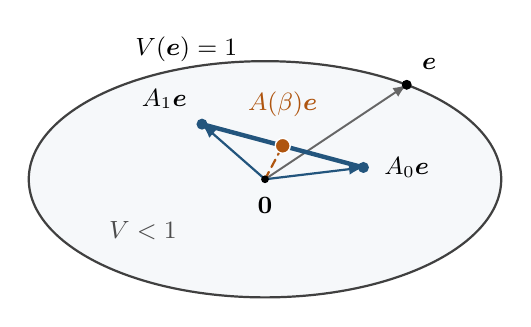
\begin{tikzpicture}[font=\small, >=latex, line cap=round, line join=round]
    \definecolor{certblue}{RGB}{35,85,125}
    \definecolor{certorange}{RGB}{175,85,15}
    \coordinate (O) at (0,0);
    \coordinate (e) at (1.8,1.2);
    \coordinate (a0) at (1.25,0.15);
    \coordinate (a1) at (-0.8,0.7);
    \coordinate (ab) at (0.225,0.425);

    \filldraw[fill=certblue!4, draw=black!75, line width=0.8pt]
        (O) ellipse [x radius=3cm, y radius=1.5cm];
    \node at (-1.0,1.65) {$V(\vect{e})=1$};
    \node[text=black!70] at (-1.55,-0.65) {$V<1$};

    \draw[->, black!60, line width=0.7pt] (O) -- (e);
    \draw[->, certblue, line width=0.8pt] (O) -- (a0);
    \draw[->, certblue, line width=0.8pt] (O) -- (a1);
    \draw[certblue, line width=1.6pt] (a0) -- (a1);
    \draw[densely dashed, certorange, line width=0.8pt] (O) -- (ab);

    \fill (O) circle [radius=1.4pt];
    \fill (e) circle [radius=1.8pt];
    \fill[certblue] (a0) circle [radius=2pt];
    \fill[certblue] (a1) circle [radius=2pt];
    \filldraw[fill=certorange, draw=white, line width=0.5pt]
        (ab) circle [radius=2.7pt];

    \node[below=3pt] at (O) {$\vect{0}$};
    \node[above right=2pt] at (e) {$\vect{e}$};
    \node[right=4pt] at (a0) {$A_0\vect{e}$};
    \node[above left=2pt] at (a1) {$A_1\vect{e}$};
    \node[above=7pt, text=certorange] at (ab) {$A(\beta)\vect{e}$};
\end{tikzpicture}
}
    \caption{Common-$P$ schematic in error coordinates. Both endpoint images lie inside the unit level set of $V$. Every intermediate image $A(\beta)\vect{e}$ lies on the segment joining them.}
    \label{fig:common-p}
\end{figure}

\begin{theorem}[Uniform stability under conditioning]
\label{thm:common-p}
Suppose there exist $P=P^{\mathsf T}\succ0$ and $\eta>0$ such that
\begin{equation}
    P-A_i^{\mathsf T}PA_i\succeq\eta I_n,\qquad i\in\{0,1\}.
    \label{eq:endpoint-lmis}
\end{equation}
Then $V(\vect{e})=\vect{e}^{\mathsf T}P\vect{e}$ decreases for every nonzero state of \eqref{eq:conditioned-family} and every $\beta\in[0,1]$. The conditioned linearized model is uniformly exponentially stable for every sequence $\{\beta_k\}\subset[0,1]$, including the state-dependent factors in \eqref{eq:conditioner}.
\end{theorem}

\begin{proof}
First, express the desired decrease $A(\beta)^{\mathsf T}PA(\beta)-P\prec0$ as a block-matrix inequality. For the same $P\succ0$ at both endpoints, define
\begin{equation}
    \mathcal S(\beta)=
    \begin{bmatrix}
        -P&A(\beta)^{\mathsf T}\\
        A(\beta)&-P^{-1}
    \end{bmatrix}.
    \label{eq:schur-block}
\end{equation}
The lower-right block is negative definite. Its Schur complement is $-P+A(\beta)^{\mathsf T}PA(\beta)$, so
\[
    \mathcal S(\beta)\prec0
    \Longleftrightarrow
    A(\beta)^{\mathsf T}PA(\beta)-P\prec0.
\]
The endpoint assumptions therefore make both $\mathcal S(0)$ and $\mathcal S(1)$ negative definite.

Next, use $A(\beta)=(1-\beta)A_0+\beta A_1$. Since the same $P$ is used throughout, the diagonal blocks do not change with $\beta$. Hence
\begin{equation}
\begin{aligned}
    \mathcal S(\beta)
    &=(1-\beta)\begin{bmatrix}
        -P&A_0^{\mathsf T}\\
        A_0&-P^{-1}
    \end{bmatrix}\\
    &\quad+\beta\begin{bmatrix}
        -P&A_1^{\mathsf T}\\
        A_1&-P^{-1}
    \end{bmatrix}\prec0.
\end{aligned}
\label{eq:schur-convex-combination}
\end{equation}
Both endpoint blocks are negative definite, and their weights are nonnegative and sum to one. Their convex combination is therefore negative definite for every $\beta\in[0,1]$.

Taking the Schur complement shows that $V(\vect{e})=\vect{e}^{\mathsf T}P\vect{e}$ decreases strictly for every nonzero error and every $\beta\in[0,1]$. The same $P$ applies throughout the interval. Since the matrix family depends continuously on $\beta$ over this compact interval, the decrease has a uniform positive margin. The quadratic Lyapunov criterion therefore establishes uniform exponential stability for any conditioning-factor sequence.
\end{proof}

In the schematic of \cref{fig:common-p}, both endpoint images and their joining segment lie inside one Lyapunov ellipsoid. The same function covers the complete factor interval and all errors of the linearized model, including those outside $\mathcal C$. This does not validate that approximation at arbitrary physical errors or define a nonlinear region of attraction.

\subsection{Offline semidefinite program}

Related common-matrix vertex-LMI formulations appear in discrete-time robust stability \cite{deOliveira1999lmiDiscrete} and in robust polytopic PWM converter control based on continuous-time averaged models \cite{olalla2009robustLqrPwm}.

The Lyapunov matrix can be computed offline, after the feedback gain $K$ has been chosen. With $A_0=\Phi_x$ and $A_1=A_{\mathrm{cl}}$ fixed, an endpoint SDP is
\begin{equation}
\begin{aligned}
    \underset{P=P^{\mathsf T},\,\eta}{\operatorname{maximize}}\quad&\eta\\
    \text{subject to}\quad
    &\operatorname{tr}(P)=n,\\
    &P\succeq\varepsilon_P I_n,\\
    &P-A_0^{\mathsf T}PA_0\succeq\eta I_n,\\
    &P-A_1^{\mathsf T}PA_1\succeq\eta I_n,
\end{aligned}
\label{eq:common-p-sdp}
\end{equation}
with $\varepsilon_P=10^{-7}$. The constraint $P\succeq\varepsilon_P I_n$ imposes a positive-definiteness floor. The trace constraint fixes the otherwise arbitrary positive scale of $P$.

For fixed endpoints, \eqref{eq:common-p-sdp} is affine in $P,\eta$ and certifies, rather than redesigns, $K$. In contrast, the proof's block form is affine in $\beta$ for fixed $P$, not in $P$ because of $P^{-1}$. Numerical solution uses the inverse-free form in scaled coordinates.

Successful solver termination is not enough to establish a certificate. We first symmetrize the returned $P$, then recompute the endpoint decrease matrices and their smallest eigenvalues:
\begin{equation}
\begin{aligned}
    Q_i&=P-A_i^{\mathsf T}PA_i,\qquad i\in\{0,1\},\\
    \mu&=\min\{\lambda_{\min}(Q_0),\lambda_{\min}(Q_1)\}.
\end{aligned}
\label{eq:verified-margin}
\end{equation}
We check that $P$ is positive definite, that its trace has the required value, and that $\mu>0$. A positive verified margin supplies the common decrease required by \cref{thm:common-p}.

The test is sufficient, not necessary. Including zero requires $A_0$ to be Schur and excludes unstable open-loop endpoints even if restricted factors could stabilize them. Failure to find a positive common margin does not establish instability.

The stability theorem applies to the conditioned linearized model. The large-error response of the exact nonlinear system, including the initially conditioned cycles, is evaluated by simulation.

\section{Application to a three-cell converter}
\label{sec:case-study}

The converter benchmark tests convergence acceleration and dwell feasibility on an already open-loop-stable plant. MPC-5 supplies a limited performance and computation reference.

\subsection{Benchmark and controller parameters}

We use the three-cell multilevel DC--DC converter benchmark of Patino et al. \cite{patino2010}. The state $\vect{x}=[v_{C_1},v_{C_2},i_L]^{\mathsf T}$ contains the two capacitor voltages and the inductor current. For binary switch commands $u_1,u_2,u_3\in\{0,1\}$, the plant matrices are
\begin{equation}
\begin{aligned}
A_{\vect{u}}&=\begin{bmatrix}
0&0&(u_2-u_1)/C_1\\
0&0&(u_3-u_2)/C_2\\
(u_1-u_2)/L&(u_2-u_3)/L&-R/L
\end{bmatrix},\\
\vect{b}_{\vect{u}}&=\begin{bmatrix}0\\0\\Eu_3/L\end{bmatrix}.
\end{aligned}
\label{eq:converter}
\end{equation}
Both $A_{\vect{u}}$ and $\vect{b}_{\vect{u}}$ depend on the switch state. The common-state-matrix reduction in \eqref{eq:marcolino-specialization} therefore does not apply. We retain the fixed nine-interval sequence $(0,1,3,7,2,0,4,7,4)$. Each physical mode ID is encoded as $4u_1+2u_2+u_3$.

The published boundaries $(0,66,88,110,132,154,220,242,264,286)$~\si{\micro\second} do not close exactly at the reported anchor $\bar{\vect{x}}(0)=(9.9247,19.2928,0.9823)^{\mathsf T}$. A one-time least-squares reconciliation preserves this anchor, the \SI{\NominalPeriodMicroseconds}{\micro\second} period, and the \SI{\BenchmarkDwellBound}{\micro\second} nominal-design bound, giving
\begin{equation}
\begin{split}
    \bar{\vect{t}}={}&(0,63.889,87.557,109.557,132.538,154.538,\\
    &218.210,240.380,263.828,286)~\si{\micro\second}.
\end{split}
\label{eq:benchmark-schedule}
\end{equation}
The full-precision schedule has closure error \NominalClosureError{} in the infinity norm and maximum boundary correction \MaximumBoundaryCorrection{}~\si{\micro\second}. This reconciles published data; reference-trajectory design is not a contribution.

\begin{table}[t]
    \centering
    \caption{Converter and timing-feedback parameters. The applied dwell bound is a simulation assumption, not a hardware-calibrated limit.}
    \label{tab:parameters}
    \begin{tabular}{ll}
        \toprule
        Quantity & Value \\
        \midrule
        Source $E$ & \SI{30}{\volt} \\
        Capacitances $C_1,C_2$ & \SI{40}{\micro\farad} \\
        Inductance $L$; resistance $R$ & \SI{10}{\milli\henry}; \SI{10}{\ohm} \\
        Intervals $N$; period $T$ & \NominalIntervalCount{}; \SI{\NominalPeriodMicroseconds}{\micro\second} \\
        Nominal-design dwell bound & \SI{\BenchmarkDwellBound}{\micro\second} \\
        Applied dwell bound $d_{\min}$ & \SI{\AppliedScheduleDwellBound}{\micro\second} \\
        State scale $S_x$ & $\operatorname{diag}(10,20,1)$ \\
        Timing scale $t_s$ & \SI{\TimingScaleMicroseconds}{\micro\second} \\
        LQR state weight $Q_n$ & $I_3$ \\
        Aggressive input weight $R_n$ & $\AggressiveInputWeight I_8$ \\
        Conservative input weight $R_n$ & $\ConservativeInputWeight I_8$ \\
        \bottomrule
    \end{tabular}
\end{table}

The schedule appears in \cref{fig:timing-mechanism}(a), and its periodic trajectory in \cref{fig:trajectories,fig:states}. The cycle averages, \SI{\CycleAverageVCOne}{\volt}, \SI{\CycleAverageVCTwo}{\volt}, and \SI{\CycleAverageIL}{\ampere}, are not feedback targets.

\subsection{Numerical scaling and feedback gains}

Using the scales in \cref{tab:parameters}, define
\begin{equation}
    \vect{z}=S_x^{-1}\vect{e},\qquad
    \widehat A_i=S_x^{-1}A_iS_x,\quad i\in\{0,1\}.
    \label{eq:normalized-endpoints}
\end{equation}
This change of coordinates leaves the endpoint eigenvalues unchanged. It is a numerical choice, not a requirement of the stability proof.

Setting $\vect{v}=\dtau/t_s$ gives the normalized timing-input matrix $B_n=S_x^{-1}\Gamma_\tau t_s$. Discrete LQR on $(\widehat A_0,B_n)$ then gives $\vect{v}^{\mathrm{raw}}=-K_n\vect{z}$. The corresponding physical-coordinate gain is $K=t_sK_nS_x^{-1}$.

The aggressive tuning uses conditioning. The conservative tuning remains dwell-feasible without it in this experiment. The nominal-design bound and smaller applied bound in \cref{tab:parameters} have distinct roles; the latter is not hardware-calibrated.

\subsection{Checking the one-cycle model}

Central finite differences of the exact map, with state steps $10^{-4}(S_x)_{ii}$ and timing step $10^{-3}t_s=\SI{0.01}{\micro\second}$, give relative Jacobian errors \PhiJacobianRelativeError{} for $\Phi_x$ and \GammaJacobianRelativeError{} for $\Gamma_\tau$. For simultaneous normalized state and timing perturbations of amplitude $\epsilon$, the residual is
\begin{equation}
\begin{split}
    r_{\mathrm{lin}}(\epsilon)=\bigl\|S_x^{-1}\bigl[&\mathcal P(\bar{\vect{x}}(0)+\Delta\vect{x},\dtau)-\bar{\vect{x}}(0)\\
    &-\Phi_x\Delta\vect{x}-\Gamma_\tau\dtau\bigr]\bigr\|_2.
\end{split}
\end{equation}
The log--log fitted slope \LinearizationResidualSlope{} agrees with the expected second-order decay.

\subsection{Numerical Lyapunov certificate}

For the aggressive gain, we apply \eqref{eq:common-p-sdp} to the normalized endpoints $\widehat A_0$ and $\widehat A_1$. Denote the resulting Lyapunov matrix by $P_n$ and the solver margin by $\eta_n$. Julia solves this problem using Convex.jl and Clarabel, with $\operatorname{tr}(P_n)=3$. The solver returns optimal status and $\eta_n=\num{\LyapunovEta}$. The normalized-coordinate matrix, shown to six decimal places, is
\begin{equation}
    P_n\approx\LyapunovMatrix.
    \label{eq:numerical-p}
\end{equation}
We then check the returned matrix rather than relying on solver status alone. Define the normalized endpoint decrease matrices
\[
    Q_{i,n}=P_n-\widehat A_i^{\mathsf T}P_n\widehat A_i,\qquad i\in\{0,1\}.
\]
Using full precision, their smallest eigenvalues and that of $P_n$ are
\begin{equation}
\begin{aligned}
    \lambda_{\min}(P_n)&=\num{\LyapunovMinEigenvalue},\\
    \lambda_{\min}(Q_{0,n})&=\num{\LyapunovEndpointZeroDecrease},\\
    \lambda_{\min}(Q_{1,n})&=\num{\LyapunovEndpointOneDecrease}.
\end{aligned}
\label{eq:numerical-margins}
\end{equation}
Both endpoint decrease margins are positive. Their minimum is $\mu_n=\num{\LyapunovDecrease}$. The reported trace and margins refer to normalized coordinates.

To connect these checks to the physical-coordinate theorem, use
\[
\begin{aligned}
    P&=S_x^{-\mathsf T}P_nS_x^{-1},\\
    P-A_i^{\mathsf T}PA_i&=S_x^{-\mathsf T}Q_{i,n}S_x^{-1}.
\end{aligned}
\]
These transformations preserve positive definiteness. Thus the numerical checks provide the physical-coordinate certificate required by \cref{thm:common-p}, without changing the feedback gain or the plant trajectories.

Python reconstructs the endpoints and Julia solves the SDP. The article pipeline independently checks them against its MATLAB model/gain and recomputes the inequalities. Full-precision and displayed rounded matrices are checked separately, using floating-point rather than interval arithmetic.

\subsection{Exact responses and dwell feasibility}

All comparison runs start from
\begin{equation}
    \vect{x}_0=[7.5143\quad20.8211\quad0.0314]^{\mathsf T},
\end{equation}
with normalized error \InitialNormalizedError{}. Exact matrix exponentials propagate the plant through its actual dwells; the linearized model is not substituted for the plant. Continuous-time curves retain 30 local samples per interval, including its end.

\begin{figure*}[t]
    \centering
    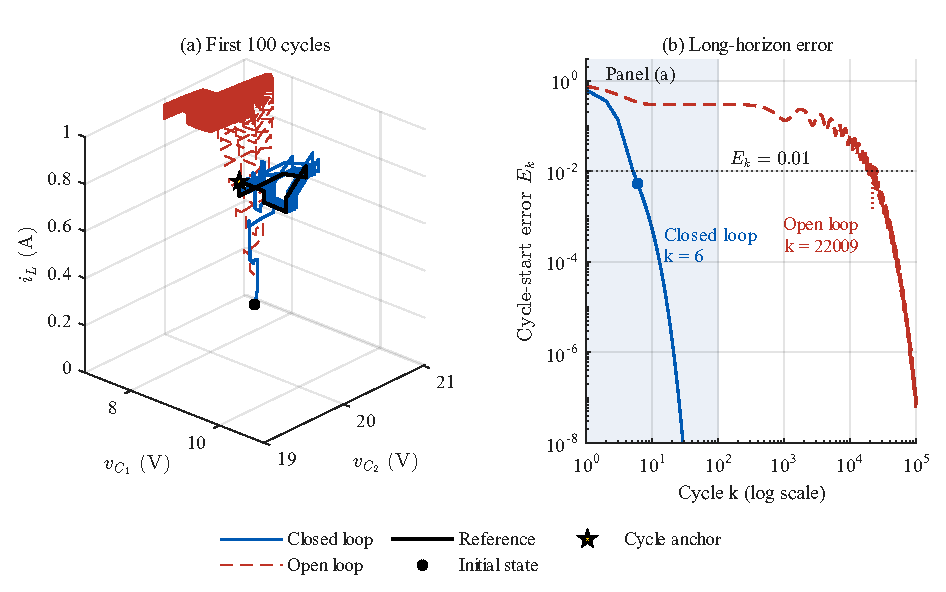
\includegraphics[width=\textwidth]{trajectory_comparison.pdf}
    \caption{Early transient and eventual convergence. (a) Continuous-time state trajectories over \SimulationCycles{} cycles. (b) Normalized cycle-start error on logarithmic axes. Shading marks the horizon in (a); dots mark the saved threshold-crossing samples.}
    \label{fig:trajectories}
\end{figure*}

In \cref{fig:trajectories}(a), feedback approaches the reference while open loop remains displaced over the same \SimulationCycles{} cycles. The dot and star mark the initial state and anchor. Panel (b) shows the much slower eventual open-loop convergence. To separate tracking error from switching ripple, report
\begin{equation}
    E_k=\bigl\|S_x^{-1}\bigl(\vect{x}(kT)-\bar{\vect{x}}(0)\bigr)\bigr\|_2,
    \label{eq:reported-cycle-error}
\end{equation}
using $S_x=\operatorname{diag}(10,20,1)$. The reporting threshold $E_k<0.01$ implies component errors below \SI{0.10}{\volt}, \SI{0.20}{\volt}, and \SI{0.01}{\ampere}; their joint norm condition is stricter than separate component bounds. It is neither a stability boundary nor a hardware accuracy requirement.

In \cref{fig:trajectories}(b), logarithmic axes omit cycle zero and errors below $10^{-8}$. Feedback extends to cycle \SimulationCycles{}, and open loop to \LongSimulationCycles{}. Markers are actual samples: the first threshold crossing for feedback and the persistent crossing through the remaining run for open loop. Neither indicates zero error.

\subsection{Conditioning and predictive-control reference}

For a computationally constrained alternative to online optimization, feasibility and a stability certificate matter alongside performance. We compare the proposed law with MPC-5 using the same initial state, cycle linearization, normalization, weights, mode sequence, period, and dwell bound. MPC optimizes eight offsets over \MpcHorizon{} cycles, applies the first action, and uses an LQR terminal cost and invariant terminal set, following the constrained predictive formulation of \cite{marcolino2021}. Its online QP has 40 variables.

\Cref{fig:response} retains the proposed controller's conditioning diagnostics while adding MPC error and applied dwell. Evaluate performance over 100 cycles using
\[
    J_{100}=\sum_{k=0}^{99}\bigl(\|S_x^{-1}\vect{e}_k\|_2^2
    +\AggressiveInputWeight\|\dtau_k^{\mathrm{app}}/t_s\|_2^2\bigr).
\]
This uses actual states and applied offsets, without the MPC terminal penalty. It is not the optimized prediction cost.

\begin{figure*}[t]
    \centering
    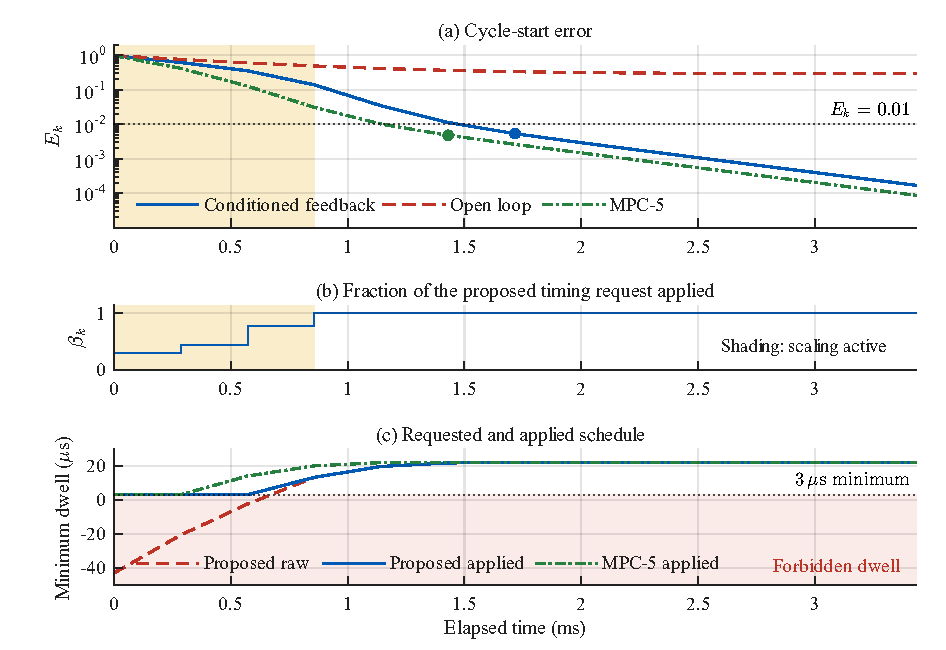
\includegraphics[width=\textwidth]{conditioned_control_response.pdf}
    \caption{First 12 cycles of the exact simulation. (a) Error and actual threshold samples. (b) Applied fraction of the proposed timing request. Shading marks active scaling. (c) Raw/applied minimum dwell, with the forbidden range shaded. MPC has no conditioning factor.}
    \label{fig:response}
\end{figure*}

\begin{table}[!htb]
    \centering
    \caption{Exact responses and matched MATLAB controller timings. Feedback thresholds are first crossings; open loop uses the persistent crossing. Costs cover 100 cycles.}
    \label{tab:results}
    \begin{tabular}{ll}
        \toprule
        Quantity & Value \\
        \midrule
        $\rho(\Phi_x)$, open loop & \OpenLoopSpectralRadius{} \\
        $\rho(A_{\mathrm{cl}})$, aggressive & \AggressiveSpectralRadius{} \\
        Spectral radius, conservative & \ConservativeSpectralRadius{} \\
        Minimum $\beta$; conditioned cycles & \MinimumConditioningBeta{}; \ConditionedCycleCount{} \\
        Maximum raw offset & \MaximumRawOffset{}~\si{\micro\second} \\
        Maximum applied offset & \MaximumAppliedOffset{}~\si{\micro\second} \\
        Minimum raw dwell & \MinimumRawDwell{}~\si{\micro\second} \\
        Minimum applied dwell & \MinimumAppliedDwell{}~\si{\micro\second} \\
        Minimum conservative dwell & \MinimumConservativeDwell{}~\si{\micro\second} \\
        Threshold cycle, conditioned & \ConditionedSettlingCycle{} \\
        Threshold cycle, conservative & \ConservativeSettlingCycle{} \\
        Persistent crossing, open loop & \OpenLoopConvergenceCycle{} \\
        \bottomrule
    \end{tabular}
    \par\smallskip
    \begin{tabular}{lrrr}
        \toprule
        Controller & $J_{100}$ & Median ($\mu$s) & p95 ($\mu$s) \\
        \midrule
        Conditioned & \ProposedEvaluationCost{} & \ProposedMatchedMedianUs{} & \ProposedMatchedPninetyfiveUs{} \\
        MPC-5 & \MpcEvaluationCost{} & \MpcMatchedMedianUs{} & \MpcMatchedPninetyfiveUs{} \\
        \bottomrule
    \end{tabular}
\end{table}

The first three factors are approximately $0.294$, $0.447$, and $0.779$. From cycle $3$, $\beta_k=1$ in this run, although feedback remains active. The raw minimum dwell, \MinimumRawDwell{}~\si{\micro\second}, is not executable. Conditioning keeps every applied dwell above the bound, attaining it whenever scaling acts, and reduces the maximum offset as reported in \cref{tab:results}. Its eventual inactivity is an observation, not a guarantee after other initial conditions or disturbances.

The conditioned and conservative laws cross the threshold at cycles \ConditionedSettlingCycle{} and \ConservativeSettlingCycle{}, respectively. MPC-5 crosses at cycle \MpcSettlingCycle{}, or \MpcSettlingMilliseconds{}~ms, and reduces $J_{100}$ by \MpcCostReduction{}\% relative to conditioned feedback. These exact-plant observations do not extend the common-$P$ guarantee beyond its linearized model.

\subsection{Periodic waveform and open-loop convergence}

\begin{figure*}[t]
    \centering
    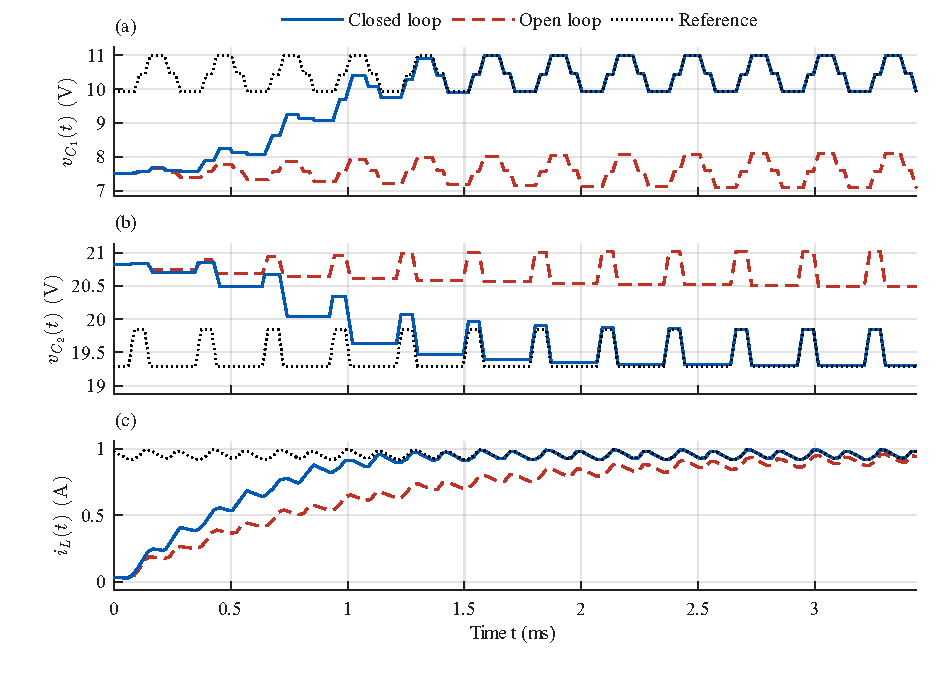
\includegraphics[width=\textwidth]{state_time_comparison.pdf}
    \caption{Continuous-time state responses over the first 12 cycles. (a) $v_{C_1}(t)$. (b) $v_{C_2}(t)$. (c) $i_L(t)$. Each panel compares closed loop, open loop, and the reference periodic waveform.}
    \label{fig:states}
\end{figure*}

In \cref{fig:states}, both responses start from the same state. Feedback approaches the repeated reference waveform while open loop remains displaced. Switching ripple belongs to the target motion, not residual tracking error; each response retains its own within-interval sample times.

For fixed nominal durations, \eqref{eq:augmented-cycle-block-form} gives $\mathcal P(\vect{x},\vect{0})=\Phi_x\vect{x}+\vect{h}$. Subtracting the fixed anchor cancels the affine term, yielding
\begin{equation}
    \vect{e}_{k+1}=\Phi_x\vect{e}_k
    \label{eq:exact-open-loop}
\end{equation}
without a remainder. Since $\rho(\Phi_x)=\OpenLoopSpectralRadius{}<1$, this fixed-schedule ideal affine model converges globally; the conclusion does not apply to nonlinear timing feedback. The \LongSimulationCycles{}-cycle open-loop simulation stays below $0.01$ from cycle \OpenLoopConvergenceCycle{} onward, over a seconds-long transient rather than the controlled response's milliseconds.

\subsection{Host computational cost}
\label{sec:computational-cost}

The matched full-controller timings in \cref{tab:results} use MATLAB R\MatchedTimingMatlabRelease{} on the same desktop and identical \MatchedTimingStates{} states: the first 12 cycle-start states of each response. After \MatchedTimingWarmup{} warm-up calls per controller, we interleave \MatchedTimingSamples{} timed calls each. The boundary includes physical error calculation, required normalization, control, schedule conversion, and feasibility checks. Offline design, plant propagation, and acquisition are excluded. First calls are recorded separately; every MPC solve starts from a zero plan, without plan reuse. The p95 is an observed percentile, not a worst-case bound.

A separate \num{\BetaTimingIndividualSamples}-call microbenchmark on an \BetaTimingCpu{} isolates conditioning. MATLAB p95 is \SI{\BetaTimingMatlabBetaPninetyfiveUs}{\micro\second} for $\beta$ alone and \SI{\BetaTimingMatlabFullPninetyfiveUs}{\micro\second} for full conditioning. Double-precision C++ with GCC \BetaTimingGccVersion{} and \texttt{-O3} reaches the \SI{\BetaTimingCppTimerFloorUs}{\micro\second} individual timer floor. Across batches of \BetaTimingBatchSize{} calls, p95 batch-average costs are \SI{\BetaTimingCppBetaBatchPninetyfiveNs}{\nano\second} for $\beta$ and \SI{\BetaTimingCppFullBatchPninetyfiveNs}{\nano\second} for conditioning, not individual latency percentiles. These desktop results neither compare C++ with MATLAB MPC nor establish embedded deadlines.

\section{Discussion}

Dwell feasibility and convergence are separate. The conditioner computes the largest feasible scale for any finite request; the offline common-$P$ test certifies the associated linearized family. Online execution needs only a fixed-gain multiplication, adjacent differences, and a minimum scan. The MPC reference illustrates this low-computation alternative with an explicit performance cost, not a general performance ranking.

The sensitivity builds on Patino et al. \cite{patino2010} and recovers Marcolino et al.'s common-state-matrix model \cite{marcolino2021}. Direction-preserving scaling also appears in control allocation \cite{nakamuraZimmerer2026directionPreserving}. The contribution is its closed form for coupled dwell inequalities and its connection to the certificate, not new LQR synthesis or a general Lyapunov theorem.

The certificate is sufficient, requires a common matrix and a Schur zero-feedback endpoint, and may fail for otherwise stable controllers. Here, feedback accelerates an already convergent open loop. Nonlinear trajectories do not certify a region of attraction. Hardware calibration of the \SI{\AppliedScheduleDwellBound}{\micro\second} bound, quantization, delays, dead time, estimation, uncertainty, and experiments remain outside scope. Desktop timings do not establish embedded feasibility.

\section{Conclusion}

An $O(N)$ scan finds the largest dwell-feasible multiple of a proportional timing action while preserving direction, mode order, and cycle period without an online solver. An offline endpoint SDP supplies a common quadratic certificate of uniform exponential stability for the conditioned linearized model under every factor sequence in $[0,1]$.

Converter simulations show feasible aggressive feedback and faster convergence than conservative feedback and the already stable open-loop schedule. Certifying the full nonlinear transient requires further analysis.

% Allow the comparison figures to share pages with the discussion,
% but keep all main-text figures before the appendix.
\FloatBarrier
\backmatter
\begin{appendices}
\section{Feasible-region expansion under timing-action scaling}
\label{app:invariant-region}

\subsection{Expansion of the dwell-feasible region}

A smaller fixed factor allows larger errors while keeping the timing action feasible. To see this, hold $\beta\in(0,1]$ fixed and apply $\dtau=-\beta K\vect{e}$. Substitution into the dwell inequalities gives the feasible region
\begin{equation}
\begin{aligned}
    \mathcal F_\beta&=\{\vect{e}:\beta DK\vect{e}\le\vect{m}\}
    =\frac{1}{\beta}\mathcal C,\\
    \mathcal F_1&=\mathcal C.
\end{aligned}
\label{eq:fixed-beta-feasible}
\end{equation}
Thus $0<\beta_a<\beta_b\le1$ gives $\mathcal F_{\beta_b}\subseteq\mathcal F_{\beta_a}$. The three-state volumes scale as $\beta^{-3}$: factors $\LowerComparisonConditioningFactor{}$, $\MiddleComparisonConditioningFactor{}$, and $1$ give volume ratios $\LowerComparisonRegionVolumeRatio{}$, $\MiddleComparisonRegionVolumeRatio{}$, and $1$. This is current-cycle feasibility, not successive-cycle stability.

\begin{figure*}[t]
    \centering
    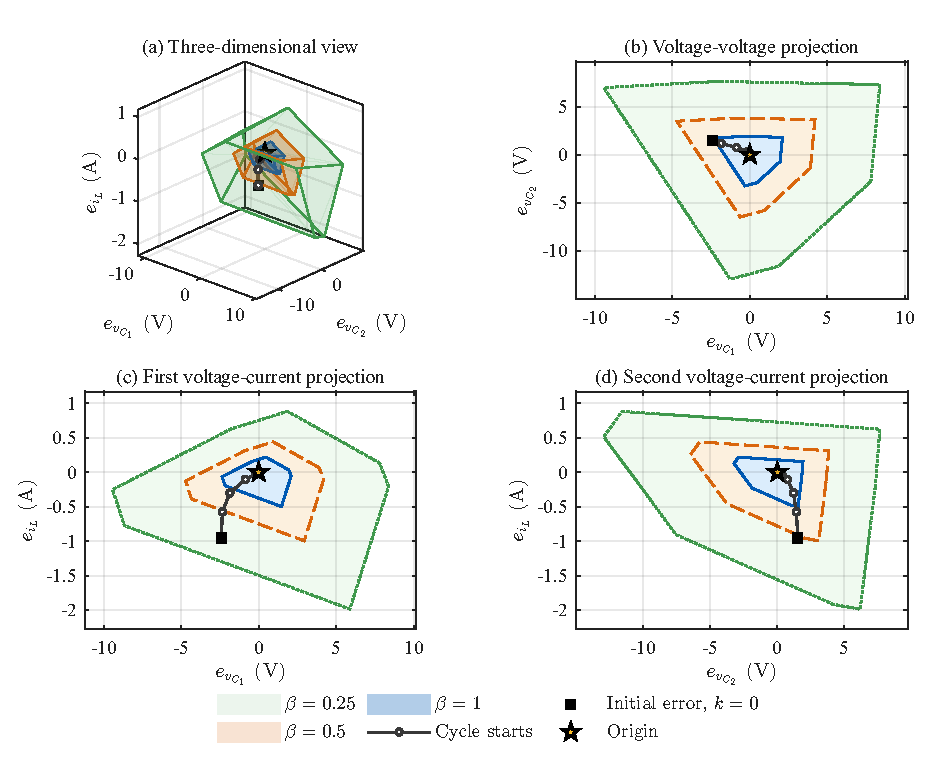
\includegraphics[width=\textwidth]{appendix_raw_action_region.pdf}
    \caption{Dwell-feasible regions for fixed factors $\beta=\LowerComparisonConditioningFactor{},\MiddleComparisonConditioningFactor{},1$, with early cycle-start errors from the conditioned simulation. (a) Three-dimensional view. (b)--(d) Coordinate-plane projections. Smaller factors admit larger errors.}
    \label{fig:appendix-region}
\end{figure*}

The overlaid simulation in \cref{fig:appendix-region} uses state-dependent, not fixed, factors. Its initial error is inside $\mathcal F_{\LowerComparisonConditioningFactor{}}$ and outside $\mathcal F_{\MiddleComparisonConditioningFactor{}}$, consistent with $\beta_0\approx0.294$; raw feasibility starts at cycle \FirstInvariantRegionCycle{}. Lines join cycle-start samples. The planar views are projections, not slices; membership uses full three-dimensional inequalities.

\subsection{Feasibility over successive cycles}

For each fixed comparison factor, the linearized dynamics are
\begin{equation}
    \vect{e}_{k+1}=M_\beta\vect{e}_k,\qquad
    M_\beta=\Phi_x-\beta\Gamma_\tau K.
    \label{eq:fixed-beta-dynamics}
\end{equation}
For all three plotted factors, offline calculations verify positive invariance,
\begin{equation}
    M_\beta\mathcal F_\beta\subseteq\mathcal F_\beta.
    \label{eq:fixed-beta-invariance}
\end{equation}
using MPT3 \cite{herceg2013mpt3} and preimage containment \cite{gilbert1991maximal}. Every vertex satisfies $\beta DK M_\beta\vect{v}\le\vect{m}$ within numerical tolerance; boundedness, convexity, and linearity extend this check to the complete polyhedron. Invariance supplies continued dwell feasibility, while \cref{thm:common-p} supplies convergence because $M_\beta=A(\beta)$.

These fixed-factor linearized checks prove neither nonlinear invariance nor an enlarged nonlinear region of attraction for state-dependent conditioning. The common-$P$ theorem does not depend on them.
\FloatBarrier
\end{appendices}

\section*{Declarations}
\textbf{Funding.} R.K.H. Galvão acknowledges the support of Conselho Nacional de Desenvolvimento Científico e Tecnológico (CNPq, Brazil) under grant 305233/2022-0.

\textbf{Competing interests.} The authors have no competing interests.

\textbf{Data availability.} Not applicable.

\textbf{Code availability.} TODO: state where the simulation and figure-generation scripts are available, or that this item is not applicable.

\textbf{Author contributions.} D. Vieira: Conceptualization; Formal Analysis; Investigation; Methodology; Software; Visualization; Writing – Original Draft Preparation. R. K. H. Galvão: Conceptualization; Formal Analysis; Investigation; Methodology; Supervision; Validation; Writing – Review \& Editing.

\textbf{ORCID.} D. Vieira: 0009-0000-3121-3269. R. K. H. Galvão: 0000-0001-9794-8815.

\bibliography{references}

\end{document}
